\chapter{Diseño e implementación del proyecto.}\label{cap:DisenhoEImplementacion}
\markboth{CAPÍTULO \ref{cap:DisenhoEImplementacion}. DISEÑO E IMPLEMENTACIÓN DEL PROYECTO.}{}
En este capítulo vamos a explicar el método elegido para el diseño de las aplicaciones del proyecto y la arquitectura que hemos tenido que diseñar para la implementación del proyecto.

\section{Metodología de diseño usada.}

La metodología usada a lo largo de todo el proyecto ha sido una metodología ágil de desarrollo. Esta metodología fue elegida ya que se basa en dar varias iteraciones y en cada iteración se va añadiendo nuevas funcionalidades al proyecto. Normalmente esta metodología se usa por equipo de programadores pero en este caso sólo estaba yo como programador y el director de proyecto fin de carrera como director del proyecto software. Al estar sólo como programador, no hemos podido aplicar ninguna de las metodologías ágiles que ya existen, por lo que hemos tomado las características generales y otras que más nos interesaban de cada una.

La característica general es que es un desarrollo iterativo e incremental. Cada uno de los periodos en los que se divide el proceso de diseño e implementación se llama etapas, que deben de tener una duración de entre una a cuatro semanas y al final de cada una debemos tener una demo funcional del proyecto, esta idea nos gustó ya que después de cada reunión añadíamos cosas nuevas al proyecto y a su vez podíamos ver como iba evolucionando.  

\section{Arquitectura del proyecto.}

La arquitectura básica del proyecto es la que podemos ver en la figura~\ref{fig:arquitecturaBasica}.

\begin{figure}
  \centering
    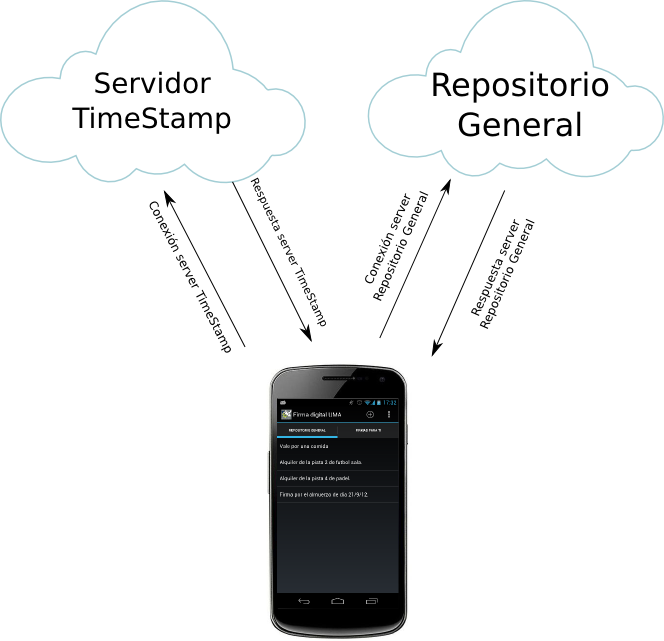
\includegraphics[scale=0.5]{./DisenhoYArquitectura/imagenes/arquitecturaBasica.png}
  \caption{Arquitectura básica del proyecto.}
  \label{fig:arquitecturaBasica}
\end{figure}

Podemos ver que la idea es tener dos aplicaciones web que son representadas por las nubes, ya que estaría en internet y una aplicación para un terminar Android. Como ya se ha explicado en capítulos anteriores en las aplicaciones web se ha usado Google App Engine para el desarrollo del proyecto y un terminar Android para la realización de las firmas. 

En la figura~\ref{fig:estructura} podemos ver la estructura final que tiene el proyecto, con las dos aplicaciones web diferenciadas y la aplicación del telefono.

\begin{figure}
  \centering
    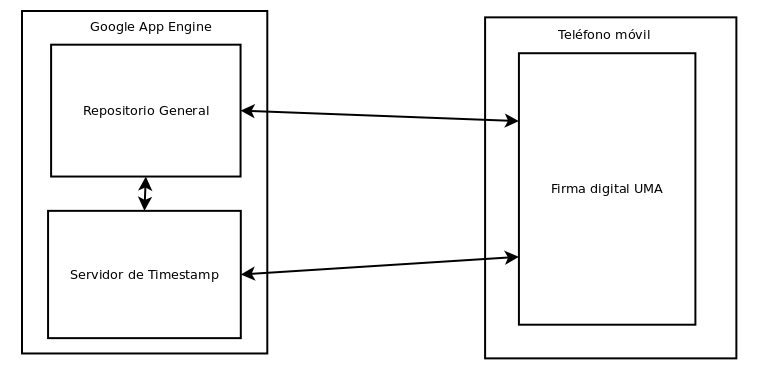
\includegraphics[scale=0.3]{./DisenhoYArquitectura/imagenes/estructura.png}
  \caption{Estructura del proyecto.}
  \label{fig:estructura}
\end{figure}

A continuación vamos a explicar cada una de las tres partes en las que se divide principalmente el proyecto.

\begin{itemize}
\item \textbf{Servidor de timestamp:} como podemos ver en la figura~\ref{fig:servertimestamp} el servidor de timestamp que hemos diseñado tiene tres partes principales, que son añadir una nueva entrada, listar una entrada determinada y listar todas las entradas para mostrarlas en la aplicación web.  
\end{itemize}

\begin{figure}
  \centering
    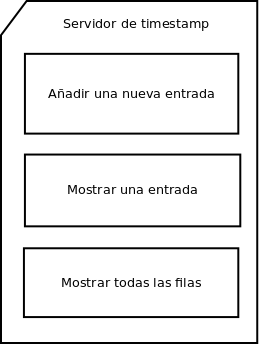
\includegraphics[scale=0.3]{./DisenhoYArquitectura/imagenes/servertimestamp.png}
  \caption{Estructura del servidor de timestamp.}
  \label{fig:servertimestamp}
\end{figure}

\begin{figure}
  \centering
    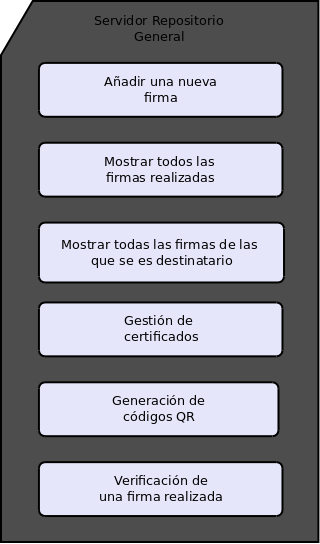
\includegraphics[scale=0.3]{./DisenhoYArquitectura/imagenes/serverRepositorioGeneral.png}
  \caption{Estructura del servidor respositorio general.}
  \label{fig:serverRepositorioGeneral}
\end{figure}

\begin{itemize}
\item \textbf{Servidor Repositorio General:} en la figura~\ref{fig:serverRepositorioGeneral} observamos la estructura básica del servidor donde tendremos el repositorio para todas las firmas realizadas y la funciones principales que nos proporciona, como pueden ser la de añadir una entrada, listar los recibos que tu has firmado o los que están dirigidos para ti, otra función importante es la gestión de certificados, la generación de código QR y la verificación de cualquier firma, para poder ver si la firma es válida o no. De todas estas funciones sólo la de añadir y las de listar ambas firmas se podrán consultar con la aplicación móvil, el resto de funciones sólo serán accesibles desde la aplicación web.  
\end{itemize}


\begin{figure}
  \centering
    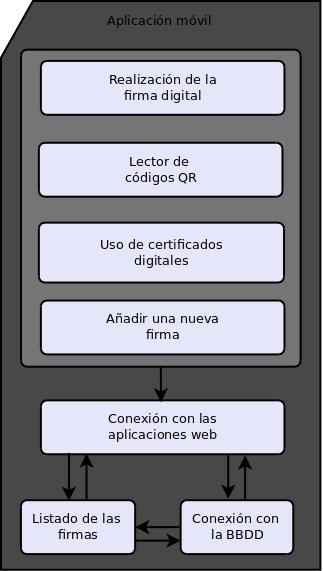
\includegraphics[scale=0.3]{./DisenhoYArquitectura/imagenes/aplicacionMovil.png}
  \caption{Estructura de la aplicación móvil.}
  \label{fig:aplicacionMovil}
\end{figure}

\begin{itemize}
\item \textbf{Aplicación Móvil:} podemos ver en la figura~\ref{fig:aplicacionMovil} la estructura general de la aplicación móvil. Como podemos observar tiene varias partes, podemos diferenciar el proceso de lectura del código QR, uso de certificados, realización de la firma digital y subirla a la aplicación web, las conexiones con las aplicaciones web, la parte de listado de las firmas y la conexión con la base de datos. Cada una de ellas tiene relación con las otras como podemos apreciar. El listado de las firmas podrá listarlas desde la base de datos o directamente de la aplicación web, dependiendo del caso en el que nos encontremos.
\end{itemize}

\section{Implementación del proyecto.}

En esta sección vamos a explicar la implementación realizada a lo largo del proyecto, tanto de la aplicación Android como de las aplicaciones web. A continuación vamos a explicar con profundidad el proyecto Android realizado.

\subsection{Proyecto Firma Digital UMA.}

La aplicación Firma Digital UMA es la aplicación móvil que hemos realizado para facilitar la firma y visualización de nuevos documentos. En ella  podemos firmar nuevos documentos o comprobar los anteriormente firmados de una forma fácil, el resto de gestiones se pueden realizar desde la aplicación web, donde se puede verificar, generar nuevos documentos para que sean firmados, etc. En la figura~\ref{fig:pantallaPrincipal} podemos ver el aspecto de la aplicación.

\begin{figure}[h]
  \centering
    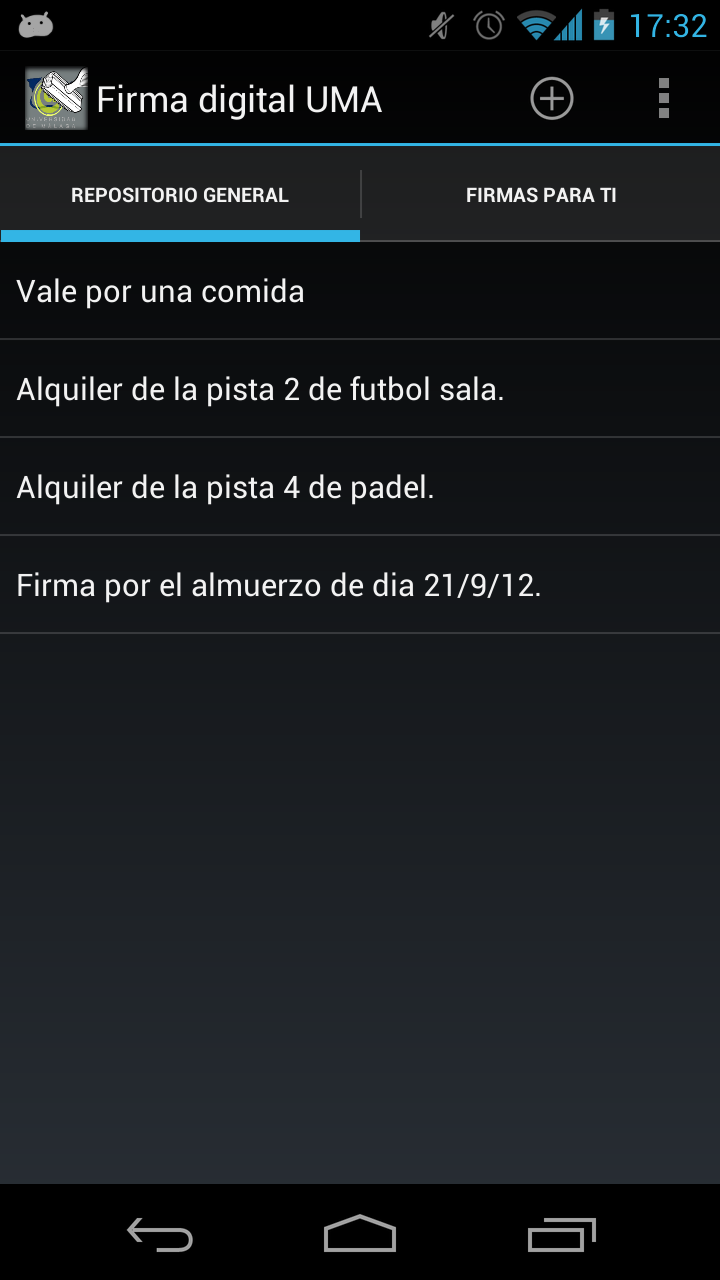
\includegraphics[scale=0.2]{./Android/imagenes/pantallaPrincipal.png}
  \caption{Pantalla inicial de la aplicación.}
  \label{fig:pantallaPrincipal}
\end{figure}

\subsubsection{Uso de la aplicación.}

Lo primero que pensamos cuando nos pusimos a diseñar la aplicación era que el método de firma tenía que ser rápido y fácil de realizar, por lo que se decidió usar los códigos QR para agilizar la lectura de información. Sólo hay que pulsar el botón de añadir nuevo recibo (figura~\ref{fig:botonAnhadir}) y se abrirá el lector de códigos QR, una vez leídos el código este se firmará y se subirá automáticamente al servidor sin necesidad de que el usuario realice otra acción.

\begin{figure}[h]
  \centering
    
\includegraphics[scale=0.2]{./Android/imagenes/botonAnhadir.png}
  \caption{Detalle del botón añadir.}
  \label{fig:botonAnhadir}
\end{figure}

La aplicación se puede dividir principalmente en dos partes claramente diferenciadas, una en la que se muestra las firmas realizadas y otra en la que se muestran que tienen como destino el usuario que está ejecutando la aplicación. Las dos partes son prácticamente idénticas y tienen el mismo uso. Si pulsamos encima de cualquier recibo de la lista nos mostrará toda la información de dicha firma, podemos ver un ejemplo en la figura~\ref{fig:informacionFirma}. Podemos observar todos los datos necesarios, como pueden ser destino, quien ha realizado la firma, la fecha, el texto, etc y también podemos ver si está verificada con el tick de color verde o una señal de error roja en caso contrario, que podemos ver en la esquina superior derecha. En el caso de los recibos de los que se es destino de la firma, se indica de una forma más clara quien es el que usuario que envía el mensaje, pero el resto de la información es la misma.

En la información que nos proporcionan podemos ver la dirección del servidor de tiempo usado y si pulsamos en ella se abrirá el navegador con una dirección donde podremos confirmar el hash y la fecha en la que se realizó la firma.

\begin{figure}
  \centering
    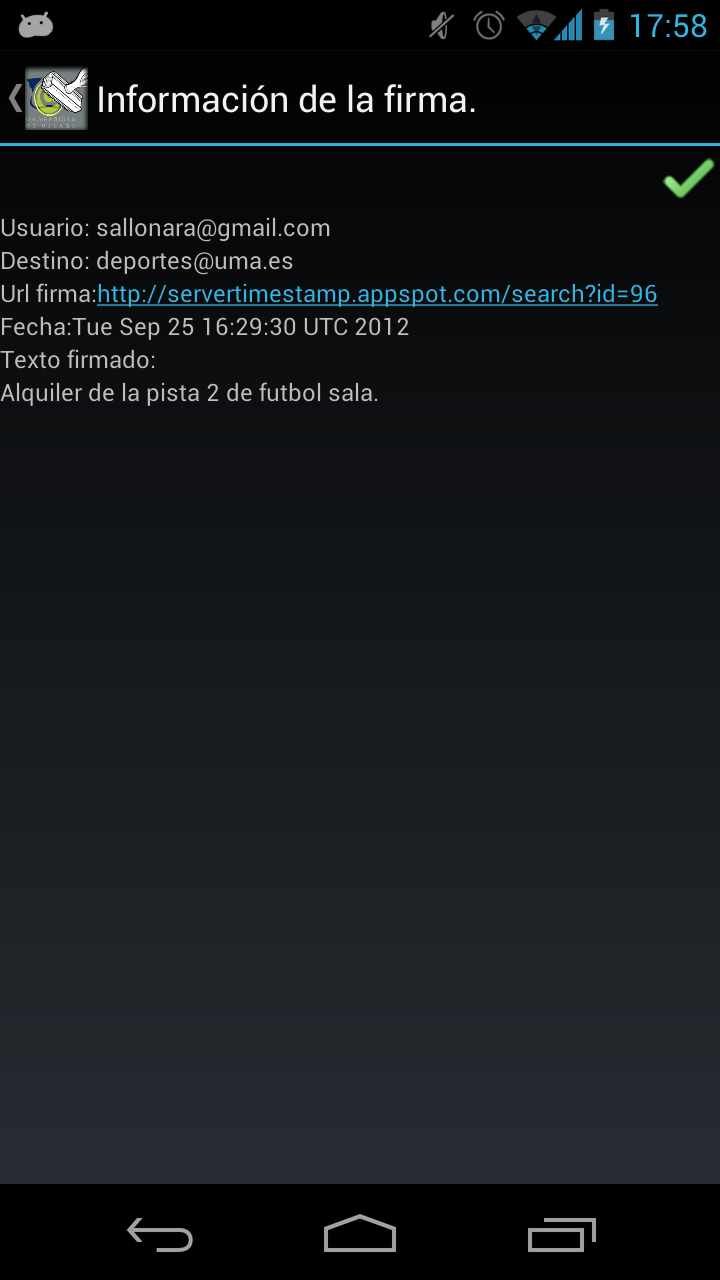
\includegraphics[scale=0.2]{./Android/imagenes/informacionFirma.png}
  \caption{Información de una firma realizada.}
  \label{fig:informacionFirma}
\end{figure}

\subsubsection{Detalles de la implementación.}

En la figura~\ref{fig:proyectoAndroid} podemos ver el proyecto de eclipse con todas las clases que hemos tenido que desarrollar, desde la conexión a la base de datos, el inicio de la aplicación, el cifrado, etc. La estructura del proyecto es la misma que ya hemos explicado anteriormente.

\begin{figure}
  \centering
    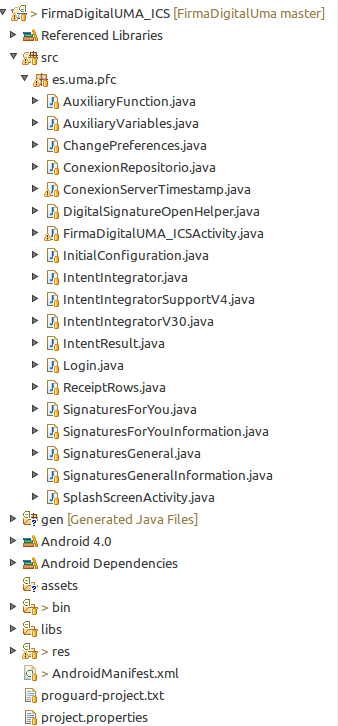
\includegraphics[scale=0.7]{./Android/imagenes/proyectoAndroid.png}
  \caption{Proyecto de Android en Eclipse.}
  \label{fig:proyectoAndroid}
\end{figure}

A continuación vamos a explicar cada una de las clases y la función que tiene dentro del proyecto.

\begin{itemize}

\item \textbf{AuxiliaryFunction.java:} en esta clase se han implementado todas las funciones que son usadas en varias clases en el proyecto, como puede ser la función que verifica si un certificado existe en un ruta determinada y si se puede abrir, también la función que pasa de un array de bytes a una cadena de texto. 

\item \textbf{AuxiliaryVariables.java:} aquí se almacenan todas las variables comunes que vamos a necesitar en la aplicación para que funcione correctamente. En el siguiente trozo de código podemos ver que son variables como el login, con el que se está autentificado, la cookie para autentificación en el servicio, el key store con las claves para realizar las firmas, si la aplicación no tiene internet, para mostrar la base de datos que tengamos almacenados y no intentar bajar recibos nuevos y otras.

\begin{lstlisting}[style=Java]
private static Login LOGIN_GLOBAL;
private static Cookie COOKIE_GLOBAL;
private static KeyStore KEYSTORE_GLOBAL;
private static boolean WITHOUT_INTERNET;
private static List<ReceiptRows> LIST_RECEIPT;
private static String THEME;
\end{lstlisting}

Además de las variables tenemos sus getter and setter correspondientes, que nos sirven para consultar o cambiar los valores.

\item \textbf{ChangePreferences.java:} esta clase es la encargada de realizar todo el manejo del cambio de preferencias, si se producen. En la aplicación hemos usado una clase que proporciona Android para el almacenado de configuración llamada \lstinline{SharedPreferences}. Al usar esta clase Android proporciona listener para que en caso de que las preferencias cambien se activen automáticamente y de esta forma podamos controlar todos los cambios que se realicen y actualizar la interfaz y guardar los cambios.

Un trozo de esta clase, en el que se puede observar como se crea y se implementa un listener que se activará cuando se produzca un cambio en la configuración lo podemos ver a continuación.

\begin{lstlisting}[style=Java]
EditTextPreference textPath = (EditTextPreference) findPreference(getActivity().getResources().getString(R.string.key_cert_path));

// Para que cuando cambie el texto lo cambie tambien en el titulo...
textPath.setOnPreferenceChangeListener(new OnPreferenceChangeListener() {
	public boolean onPreferenceChange(Preference preference, Object newValue) {
		EditTextPreference textPath = (EditTextPreference) preference;
		String s = (String) newValue;

		String pass = settings.getString("certificate_password", "NotValue");
		if (!pass.equals("NotValue")) {
			boolean check = AuxiliaryFunction.checkCert(s, pass);

			if (check) {
				textPath.setSummary(s);
				textPath.setText(s);
				Editor editor = settings.edit();
				editor.putString("path_certificate", s);
				editor.commit();
				return true;
			} else {
				textPath.setSummary("No se ha podido cargar el certificado,\nla ruta no es correcta");
				return true;
			}
		} else {
			textPath.setSummary("Password no guardado");
			return true;
		}

	}

});
\end{lstlisting}

Creamos la variable EditTextPreference donde mostraremos el password del certificado que estamos usando para firmar el texto. A continuación implementamos el listener \lstinline{OnPreferenceChangeListener}, el cual se activará cuando cambiemos el password del certificado. Podemos observar que cuando introducimos un nuevo password hacemos una comprobación para ver si después del cambio podemos seguir usando dicho certificado, si no es posible informamos al usuario mostrando un mensaje en el que se le indicará que no se ha guardado el password.

\item \textbf{ConexionRepositorio.java:} en esta clase se ha implementado todo lo referente a interactuar con la aplicación web Repositorio General. En dicha clase se ha implementado el método para añadir un recibo nuevo, listar todos los recibos que hay guardados, etc. Todos los métodos son estáticos para no tener que crear instancias de esta clase, además se vio que teníamos que crear una nueva conexión cada vez que queríamos añadir un nuevo recibo, por lo que no tendría sentido crea instancias de esta clase. A continuación podemos ver el método que añade un nuevo recibo.

\begin{lstlisting}[style=Java]
public static String addRow(String plainText, String tokenTime, Account account, String to) {
	/*
	 * Primero se le codifican los espacios porque si no la funcion
	 * URLEncoder.encode los cambia por '+' y si el documento tiene '+'
	 * luego los pone como si fueran espacios
	 */
	String textoSinEspacios = plainText.replace(" ", "%20");
	textoSinEspacios = URLEncoder.encode(textoSinEspacios);
	String token = tokenTime.split(";;")[1];
	String fecha = tokenTime.split(";;")[2];
	String url = cadServer + cadAdd + cadServerTimestampSearch + token + "&texto=" + textoSinEspacios + "&token=" + token + "&usuario=" + account.name
			+ "&destino=" + to + "&fecha="+ fecha;
	String response = "";
	try {
		URL u1 = new URL(url);

		// Si queremos usar el proxy inicializarlo de esta forma, donde
		// sa es: SocketAddress sa = new
		// InetSocketAddress("proxy.alu.uma.es", 3128);
		// HttpURLConnection c = (HttpURLConnection)
		// u.openConnection(new Proxy(Proxy.Type.HTTP, sa));

		Cookie cookie = AuxiliaryVariables.getCOOKIE_GLOBAL();
	
		HttpURLConnection con1 = (HttpURLConnection) u1.openConnection();

		con1.addRequestProperty("Cookie", cookie.getName() + "=" + cookie.getValue());
		con1.setRequestMethod("GET");
		con1.connect();

		DataInputStream is1 = new DataInputStream(con1.getInputStream());
		response = is1.readLine();

		con1.disconnect();

	} catch (MalformedURLException e) {
		response = "MalformedURL";
		e.printStackTrace();
	} catch (ProtocolException e) {
		response = "ProtocolException";
		e.printStackTrace();
	} catch (IOException e) {
		response = "IOException";
		e.printStackTrace();
	}
	return response;
}
\end{lstlisting}

La función necesita una serie de parámetros para poder ser invocada, estos parámetros son los datos que queremos almacenar, como pueden ser el texto en claro, el token de tiempo que ha devuelto la aplicación web de timestamp, la cuenta con la que se está usando la aplicación y el destino, el resto de valores o los añade la aplicación web o la aplicación del móvil. A continuación se realiza la conexión con el servidor y se recibe una cadena donde se indica si se ha realizado bien la operación.

\item \textbf{ConexionServerTimestamp.java:} al igual que la clase anterior en esta se ha realizado todo lo relacionado con la conexión con la aplicación web del Servidor Timestamp. Sólo tiene una función que es la de añadir al servidor, que tiene un aspecto similar a la mostrada en el apartado anterior.

\item \textbf{DigitalSignatureOpenHelper.java:} esta clase es la encargada de la creación de la base de datos SQLite, cuando vamos a necesitar tener acceso a ella hay que generar un objeto de dicha clase y llamar al constructor, que devuelve un objeto con el que podremos buscar, insertar o borrar elementos de la base de datos. Al pensar en el diseño de la aplicación se creyó necesario el uso de la base de datos para almacenar todos los recibos que se han realizado hasta la fecha, la aplicación sabe cual es el último recibo que tiene almacenado y sólo pide a la aplicación web que le de los recibos nuevos, de esta forma de ahorra en tiempo de inicio de la aplicación y además en la cantidad de datos móviles que usamos.

Esta clase tiene que heredar de \lstinline{SQLiteOpenHelper} que es la clase genérica que proporciona Android para manejo de la base de datos SQLite que tiene. Hay que implementar el constructor y dos métodos más obligatoriamente \lstinline{public void onCreate(SQLiteDatabase db);} y \lstinline{public void onUpgrade(SQLiteDatabase db, int oldVersion, int newVersion);}, el primero es usado para crear la base de datos en la primera ejecución y el segundo para actualizar la base de datos cuando sea necesario.

La base de datos se crea con la siguiente sentencia SQL, podemos verla en el siguiente trozo de código.

\begin{lstlisting}[style=Java]
static final String KEY_SEQ_NUM = "NUM_SEC";
static final String KEY_SIGN_URL = "URL_FIRMA";
static final String KEY_PLAIN_TEXT = "TEXTO_CLARO";
static final String KEY_TIME_TOKEN = "TOKEN_TIEMPO";
static final String KEY_USER = "USUARIO";
static final String KEY_VERIFY = "VERIFICADO";
static final String KEY_DESTINY = "DESTINO";
static final String KEY_DATE = "FECHA";

private static final String DIGITALSIGNATURE_TABLE_CREATE = "CREATE TABLE " + DIGITALSIGNATURE_TABLE_NAME + " (" +
	BaseColumns._ID + " INTEGER PRIMARY KEY AUTOINCREMENT," +
	KEY_SEQ_NUM + " TEXT, " +
	KEY_SIGN_URL + " TEXT, " +
	KEY_PLAIN_TEXT + " TEXT, " +
	KEY_TIME_TOKEN + " TEXT, " +
	KEY_USER + " TEXT, " +
	KEY_VERIFY + " TEXT, " +
	KEY_DESTINY + " TEXT, " +
	KEY_DATE + " TEXT );";
\end{lstlisting}

\item \textbf{FirmaDigitalUMA\_ICSActivity.java:} esta es la clase principal del proyecto, en ella se crea la activity principal de la aplicación. Se puede ver en el código que no extiende a la clase \lstinline{Activity}, si no que lo hace de \lstinline{FragmentActivity}, esto es así porque como ya hemos explicado anteriormente se han usado \lstinline{Fragment} para el diseño de la aplicación y no sólo \lstinline{Activity}. Además de esto se ha añadido funcionalidad mediante el uso de \lstinline{ViewPager} y \lstinline{TabsAdapter}, el primero para el uso del scroll lateral y el segundo para tener las dos pestañas principales de la aplicación. En el siguiente trozo de código podemos ver la creación de los dos elementos que hemos dicho antes, junto con la action bar.

\begin{lstlisting}[style=Java]
mViewPager = new ViewPager(this);
mViewPager.setId(R.id.pager);
setContentView(mViewPager);

final ActionBar bar = getActionBar();
bar.setTitle("Firma digital UMA");
bar.setNavigationMode(ActionBar.NAVIGATION_MODE_TABS);

mTabsAdapter = new TabsAdapter(this, mViewPager);
mTabsAdapter.addTab(bar.newTab().setText("Repositorio general"), SignaturesGeneral.class, null);
mTabsAdapter.addTab(bar.newTab().setText("Firmas para ti"), SignaturesForYou.class, null);
\end{lstlisting}

Además de la creación de los elementos anteriores esta clase también es la encargada de crear los menús, que en la versión 4.0 de Android tienden a desaparecer debido a la desaparición del botón físico de menú en los nuevos terminales. En las nueva versión el botón de menú se añade a la action bar, junto con las acciones más importantes. A continuación podemos ver como se crean y añaden los botones de añadir un nuevo recibo, el de configuración o el de salir de la aplicación.

\begin{lstlisting}[style=Java]
@Override
public boolean onCreateOptionsMenu(Menu menu) {
	MenuInflater inflater = getMenuInflater();
	inflater.inflate(R.menu.main, menu);
	return true;
}
@Override
public boolean onOptionsItemSelected(MenuItem item) {
	switch (item.getItemId()) {

	case R.id.menuitem_add:
		Log.d(AuxiliaryVariables.TAG_DEBUG, "Add");
		IntentIntegrator intentQR = new IntentIntegrator(this);
		intentQR.initiateScan();
		return true;

	case R.id.menuitem_quit:
		Log.d(AuxiliaryVariables.TAG_DEBUG, "Quit");
		finish();
		return true;
	case R.id.menuitem_about:
		Log.d(AuxiliaryVariables.TAG_DEBUG, "About");
		Toast.makeText(context, "about", Toast.LENGTH_SHORT).show();
		return true;
	case R.id.menuitem_settings:
		Log.d(AuxiliaryVariables.TAG_DEBUG, "Settings");
		Toast.makeText(context, "ajustes", Toast.LENGTH_SHORT).show();
		Intent prefsIntent = new Intent(getApplicationContext(),
		        ChangePreferences.class);
		startActivity(prefsIntent);
		return true;
	}
	return false;
}
\end{lstlisting}

Además de la creación de la activity y de los menús es la encargada de llamar a la función de subir un recibo a la aplicación web después de recibir por medio de un intent el resultado de la lectura del código QR, se puede ver en este trozo de código.

\begin{lstlisting}[style=Java]
public void onActivityResult(int requestCode, int resultCode, Intent intent) {
	IntentResult scanResult = IntentIntegrator.parseActivityResult(requestCode, resultCode, intent);
	String plaintext = "";
	if ((plaintext = scanResult.getContents()) != null) {
		progressDialog = new ProgressDialog(activity);
		progressDialog.setMessage("Subiendo el recibo...");
		progressDialog.show();

		ConexionRepositorio.addRow(handler, plaintext);
		
	}
}
\end{lstlisting} 

\item \textbf{InitialConfiguration.java:} esta clase es la encargada de realizar la configuración de la aplicación cuando es la primera ejecución en un teléfono, en ella se tiene que configurar el certificado y su password y la cuenta. Es la encargada de crear las \lstinline{SharedPreferences} para que la aplicación funcione correctamente.

\item \textbf{InitialConfiguration.java, IntentIntegratorSupportV4.java, IntentIntegratorV30.java, IntentResult.java:} estas clases son las encargadas de la lectura de los códigos QR. Están hechas por ZXing y se distribuyen bajo licencia Apache License, Version 2.0. Proporcionan mediante un intent la posibilidad de lectura de códigos QR con su aplicación Barcode Scanner (figura~\ref{fig:barcodeScanner}) gratuita en Google Play, si no se tiene la aplicación instalada proporciona los métodos para hacerlo.

\end{itemize}

\begin{figure}[h]
  \centering
    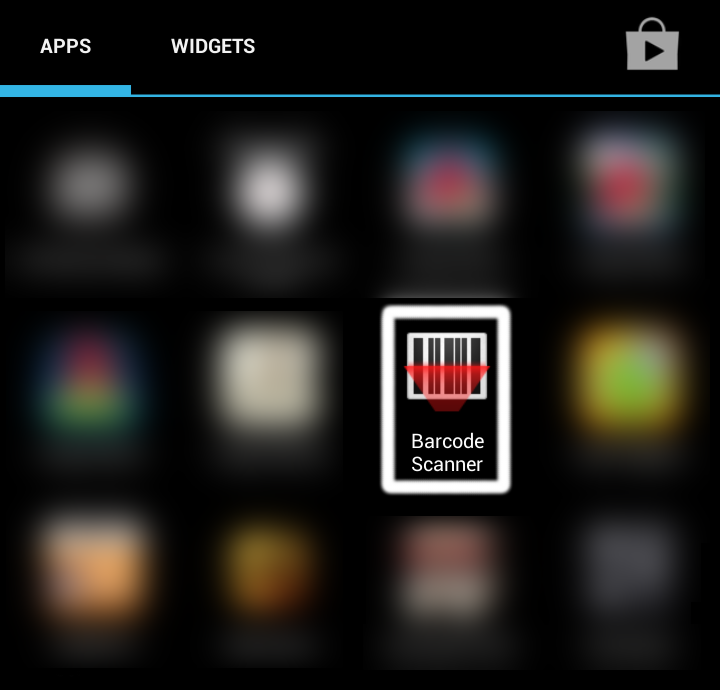
\includegraphics[scale=0.3]{./Android/imagenes/barcodeScanner.png}
  \caption{Aplicación Barcode Scanner.}
  \label{fig:barcodeScanner}
\end{figure}

\begin{itemize}

\item \textbf{Login.java:} esta clase es la encargada de realizar el login en la aplicación web Repositorio General. Google proporciona un método de login si se tienen las credenciales, cosa que tenemos gracias a que en Android se necesita tener una cuenta de Google para poder usar Google Play y los diferentes servicios que ofrece. La dirección a la que tenemos que dirigirnos es a: \url{https://repositoriorecibos.appspot.com/\_ah/login}. Esta clase tiene una variable privada que es el token de autentificación que conseguimos mediante la realización del login, para conseguirlo mostramos todas las cuentas de Google que hay configuradas en el terminal Android, cuando el usuario selecciona una de ellas iniciamos la conexión con el servidor y recibimos el token. Esto se hace todo en segundo plano para que la aplicación no se quede parada mientras se realiza el proceso de obtención del token. En el código que sigue podemos ver el proceso de obtención del token.

\begin{lstlisting}[style=Java]
Thread t = new Thread() {
	public void run() {
		try {
			AccountManagerFuture<Bundle> future = manager.getAuthToken(account, "ah", null, activity, null, null);
			Bundle bundle;
			bundle = future.getResult();
			token = bundle.getString(AccountManager.KEY_AUTHTOKEN);
		} catch (OperationCanceledException e) {
			e1.printStackTrace();
		} catch (AuthenticatorException e) {
			e1.printStackTrace();
		} catch (IOException e) {
			e1.printStackTrace();
		}
	}
}.start();
\end{lstlisting} 

La parte más interesante del código es en la llamada \lstinline{manager.getAuthToken(account, "ah", null, activity, null, null);} con esta función conseguimos la cookie donde está el token de acceso para posteriormente con la función \lstinline{bundle.getString(AccountManager.KEY_AUTHTOKEN);} conseguirlo.

La función \lstinline{public Cookie getAuthCookie(String authToken);} se puede ver en el siguiente trozo de código.

\begin{lstlisting}[style=Java]
public Cookie getAuthCookie(String authToken) throws ClientProtocolException, IOException {
	DefaultHttpClient httpClient = new DefaultHttpClient();
	Cookie retObj = null;
	String cookieUrl = gaeAppLoginUrl + "?continue=" + URLEncoder.encode(gaeAppBaseUrl, "UTF-8") + "&auth=" + URLEncoder.encode(authToken, "UTF-8");
	
	HttpGet httpget = new HttpGet(cookieUrl);
	HttpResponse response = httpClient.execute(httpget);
	if (response.getStatusLine().getStatusCode() == HttpURLConnection.HTTP_OK
			|| response.getStatusLine().getStatusCode() == HttpURLConnection.HTTP_NO_CONTENT) {

		if (httpClient.getCookieStore().getCookies().size() > 0) {
			retObj = httpClient.getCookieStore().getCookies().get(0);
		}

	}

	return retObj;
}
\end{lstlisting} 

En ella podemos ver que hacemos una conexión a la dirección \url{http://repositoriorecibos.appspot.com/\_ah/login?continue=http://repositoriorecibos.appspot.com&auth=token}, en la que se le indica el token de acceso y la url a la que tenemos que seguir cuando se realice el login. Una vez realizada la identificación devolvemos la cookie donde irá el token de acceso.

\item \textbf{ReceiptRows.java:} esta clase es la que representa un recibo, con ella se pueden crear objetos para almacenar todos los valores que necesitamos para identificar un recibo, como pueden ser el texto, la url de la firma, la fecha, el destino, etc. Este es el tipo de objeto que se usa para recoger la información de la base de datos y para almacenarla. Durante toda la ejecución de la aplicación tendremos una lista de objetos de esta clase para tener acceso a los recibos. Es una clase simple con un constructor con todos los valores que se guardan como parámetros y los getter y setter de las diferentes variables. También tiene definidas todas las constantes para el nombre de la tabla de la base de datos.

\item \textbf{SignaturesGeneral.java:} esta clase extiende a \lstinline{ListFragment}, es la lista de los recibos que el usuario a firmado. Es una de las dos pantallas principales de la aplicación, se puede ver en la figura~\ref{fig:signaturesGeneral}. Cuando se genera la interfaz se hace una consulta a la base de datos y se recibe un objeto de la clase \lstinline{Cursor}, con el que se puede iterar para obtener todos los recibos que ha firmado el usuario. En el siguiente trozo de código podemos ver como se hace.

\begin{lstlisting}[style=Java]
DigitalSignatureOpenHelper digitalSignatureOpenHelper = new DigitalSignatureOpenHelper(activity);
SQLiteDatabase sqLiteDatabase = digitalSignatureOpenHelper.getReadableDatabase();
Cursor cursor = sqLiteDatabase.query(DigitalSignatureOpenHelper.DIGITALSIGNATURE_TABLE_NAME,new String[] { DigitalSignatureOpenHelper.KEY_PLAIN_TEXT }, null, null, null, null, null);
\end{lstlisting} 

%\end{itemize}

\begin{figure}[h]
  \centering
    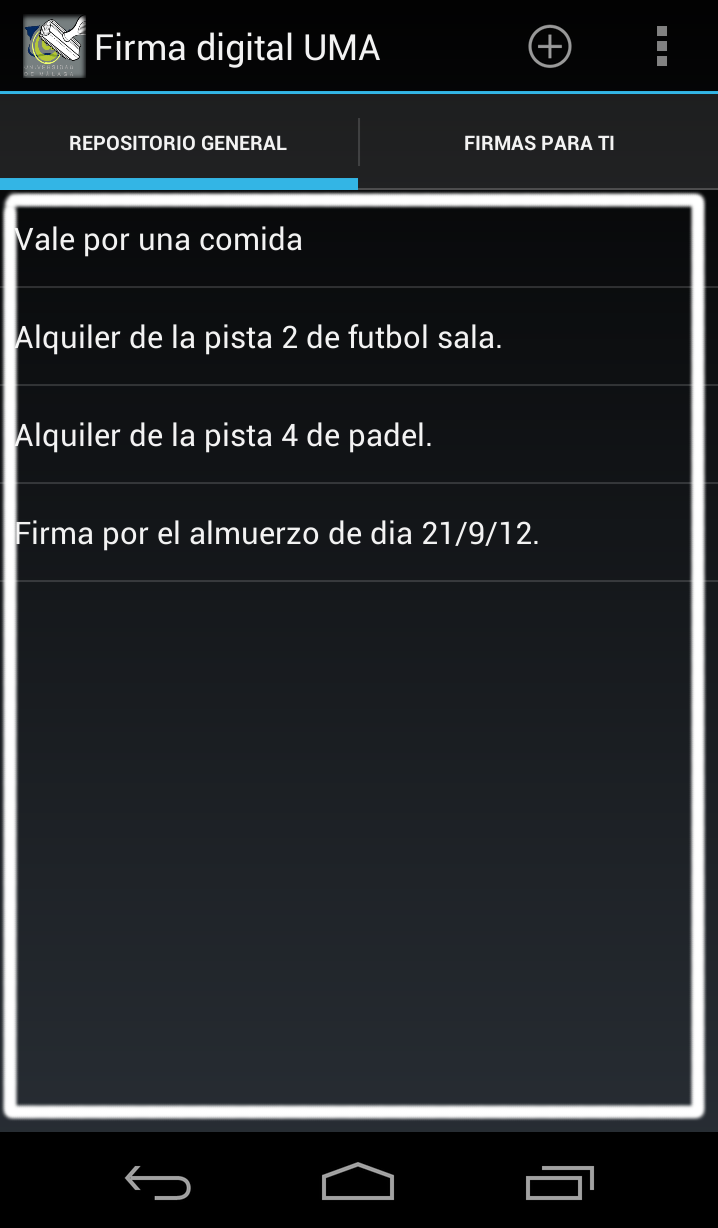
\includegraphics[scale=0.2]{./Android/imagenes/signaturesGeneral.png}
  \caption{Detalle fragment generado por la clase SignaturesGeneral.java.}
  \label{fig:signaturesGeneral}
\end{figure}

%\begin{itemize}

\item \textbf{SignaturesGeneralInformation.java:} esta clase es la encargada de mostrar la información cuando pulsamos en algún recibo que hemos firmado. Es una clase que extiende de la clase \lstinline{Activity} y es la encargada de cargar la interfaz modelada en el XML \lstinline{signaturesgeneralinfo.xml} y mostrar toda la información del recibo que ha sido pulsado de la lista. Cuando se pulsa un recibo en la pantalla anterior que es la generada por \lstinline{SignaturesGeneral.java}, antes de cargar esta se le manda la posición que ha sido pulsada para después poder localizarla y acto seguido se muestra la información, esto se hace por medio de un \lstinline{Intent} al cual se le añade un valor entero con la posición. En el siguiente trozo de código podemos ver como se recupera el valor, se realiza la consulta en la base de datos y se rellenan todos los campos donde mostraremos la información del recibo seleccionado.

\begin{lstlisting}[style=Java]
super.onCreate(savedInstanceState);
setContentView(R.layout.signaturesgeneralinfo);

Intent intent = this.getIntent();
int pos = intent.getExtras().getInt("position");

DigitalSignatureOpenHelper digitalSignatureOpenHelper = new DigitalSignatureOpenHelper(this);
SQLiteDatabase sqLiteDatabase = digitalSignatureOpenHelper.getReadableDatabase();
Cursor cursor = sqLiteDatabase.query(DigitalSignatureOpenHelper.DIGITALSIGNATURE_TABLE_NAME, new String[] { DigitalSignatureOpenHelper.KEY_USER, DigitalSignatureOpenHelper.KEY_DESTINY, DigitalSignatureOpenHelper.KEY_SIGN_URL, DigitalSignatureOpenHelper.KEY_PLAIN_TEXT, DigitalSignatureOpenHelper.KEY_VERIFY, DigitalSignatureOpenHelper.KEY_DATE }, null, null, null, null, null);

if (cursor.moveToPosition(pos)) {
	
	final ActionBar bar = getActionBar();
	bar.setTitle("Informacion de la firma.");
	bar.setDisplayHomeAsUpEnabled(true);

	TextView textUser = (TextView) findViewById(R.id.text_sign_general_user);
	TextView textDestiny = (TextView) findViewById(R.id.text_sign_general_to);
	TextView textUrl = (TextView) findViewById(R.id.text_sign_general_url);
	TextView textPlainText = (TextView) findViewById(R.id.text_sign_general_plain_text);
	ImageView imageVerify = (ImageView) findViewById(R.id.image_sign_general_verify);
	TextView textDate = (TextView) findViewById(R.id.text_sign_general_date);
	
	textUser.setText(textUser.getText() + " " + cursor.getString(0));
	textDestiny.setText(textDestiny.getText() + " " + cursor.getString(1));
	textUrl.setText(cursor.getString(2));
	textPlainText.setText(cursor.getString(3));

	String verify = cursor.getString(4);
	if (verify.equals("true")) {
		imageVerify.setImageResource(R.drawable.ok);
	} else {
		imageVerify.setImageResource(R.drawable.cancel);
	}
	textDate.setText(cursor.getString(5));

	sqLiteDatabase.close();
}
\end{lstlisting} 

Podemos ver como se genera el objeto \lstinline{DigitalSignatureOpenHelper} y se realiza la consulta con el método \lstinline{public Cursor query(String table, String[] columns, String selection, String[] selectionArgs, String groupBy, String having, String orderBy);}, a continuación generamos todos los \lstinline{TextView} necesarios para mostrar la información y los rellenamos con los datos.

\item \textbf{SignaturesForYou.java:} esta clase desarrollada es equivalente a la clase \lstinline{SignaturesGeneral.java} y es la encargada de mostrar una lista con todos los recibos de los que el usuario es destinatario, la estructura es prácticamente idéntica, con una única diferencia y es que se realiza un filtrado para que el campo destino sea el mismo que la cuenta de usuario usada en la aplicación. Podemos ver el resultado en la figura~\ref{fig:signaturesForYou}.

%\end{itemize}

\begin{figure}[h]
  \centering
    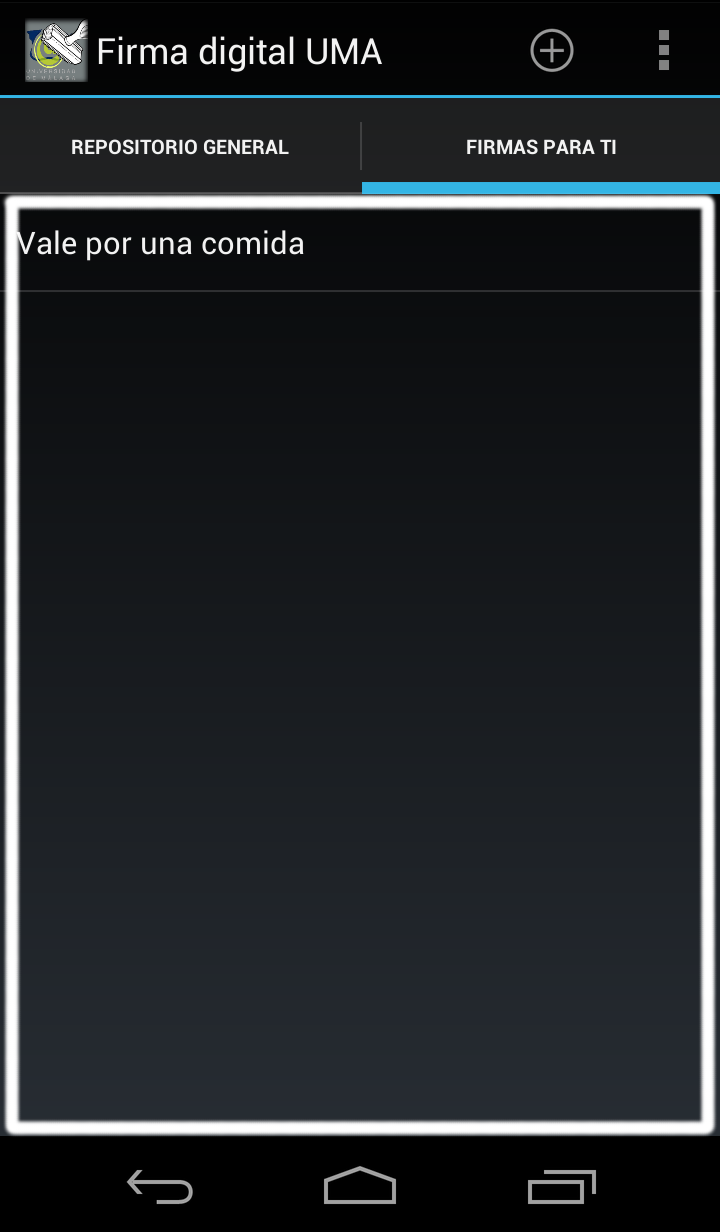
\includegraphics[scale=0.2]{./Android/imagenes/signaturesForYou.png}
  \caption{Detalle fragment generado por la clase SignaturesForYou.java.}
  \label{fig:signaturesForYou}
\end{figure}

%\begin{itemize}

\item \textbf{SignaturesForYouInformation.java:} es equivalente a la clase \lstinline{SignaturesGeneralInformation.java} y es la encargada de mostrar la información de los recibos que van dirigidos al usuario. El proceso es igual que en \lstinline{SignaturesGeneralInformation.java}, se envía la posición que ha sido marcada y se busca dicho recibo y se muestra toda la información.

\item \textbf{SplashScreenActivity.java:} esta clase es la encargada de generar la primera activity que se muestra en la aplicación cuando se inicia, además de cargar todas las variables que serán usadas durante la ejecución. Esta clase crea una interfaz en la que sólo muestra el logo de la aplicación y una barra progreso que muestra el proceso de carga, pero en background comprueba que no sea la primera ejecución, si lo es llama a la clase \lstinline{InitialConfiguration.java} para generar la configuración. Si no es la primera ejecución abre el archivo de preferencias compartidas y genera todos los objetos necesarios para la ejecución como pueden ser, la cuenta que utilizaremos posteriormente, el tema que estamos usando, hace el login en la aplicación web, el keystore que usaremos para firmar en la aplicación y a parte realizamos la conexión con la aplicación web Repositorio General y conseguimos las filas que se hayan insertado nuevas añadiéndolas a la base de datos de la aplicación para que posteriormente podamos usarlas sin tener que pedirlas al servidor, para ello se utiliza un objeto de tipo \lstinline{JSONArray}, una vez realizadas todas esas acciones se procede a la inicialización de una nueva activity que genera la clase \lstinline{FirmaDigitalUMA_ICSActivity.java} y que dará lugar a la creación de la interfaz principal de la aplicación.

\end{itemize}

A continuación vamos a explicar las dos aplicaciones web realizadas.

\subsection{Servidor de timestamp.}

En este apartado vamos a explicar en profundidad todo lo relacionado con la aplicación de timestamp que he tenido que desarrollar, desde el diseño que se ha seguido hasta los problemas que me han surgido.

En principio me gustaría explicar para que se usa un servidor de timestamp en general. Un servidor de timestamp es un registro donde cualquier persona puede subir un documento y el servidor guarda ese documento añadiéndole la fecha en la que se realizó la subida, dicha aplicación luego ofrece el servicio de consultar a que hora fue subido dicho documento. Un ejemplo podría ser \url{https://seguro.ips.es/servidortimestamp/index.asp} que se puede ver una captura de pantalla en la figura~\ref{fig:server_ips_timestamp}. En dicha captura podemos ver que tiene las opciones básicas de un servidor de timestamping como puede ser generar un sello, consultar su validez, etc. 

\begin{figure}[h]
  \centering
    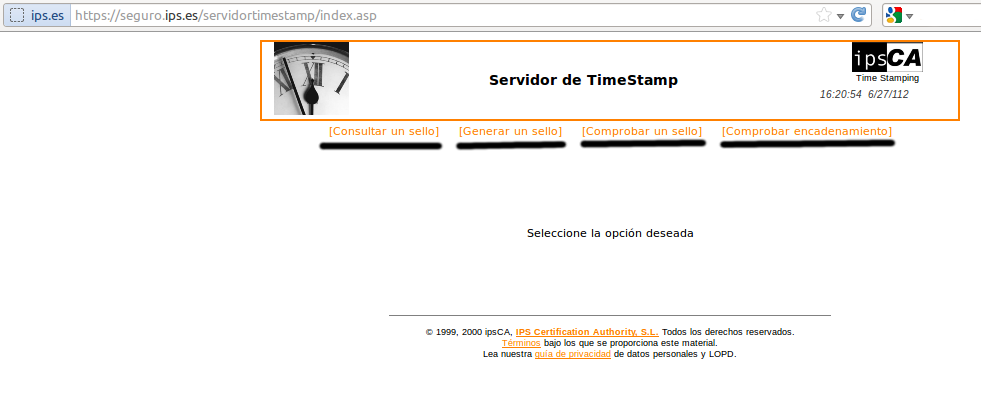
\includegraphics[scale=0.5]{./GoogleAppEngine/imagenes/server_ips_timestamp.png}
  \caption{Servidor Timestamp https://seguro.ips.es/servidortimestamp}
  \label{fig:server_ips_timestamp}
\end{figure}

La veracidad de que el sellado de dicho documento fue en el instante que dice ser, depende de la confianza que se tenga en ese servicio. Es similar a cuando se necesita que te sellen un documento físico, que dependiendo de quien lo necesite, necesitamos que lo firme un notario, un empleado público, etc. Normalmente suelen existir servidores de timestamping en los que se tiene confianza y los documentos sellados se consideran verdaderos.

Existen tres modelos principales de servidor de timestamping que son los siguientes:

\begin{itemize}

\item \textbf{Solución Arbitrada básica:} En esta solución el usuario que quiere sellar algo mandaría una copia del documento que quiere sellar a la entidad de sellado, que pondría el sello de tiempo y guardaría una copia de dicho documento, este es el modelo más parecido a la vida real. Esta solución tiene un par de grandes problemas como puede ser la privacidad del documento que se pierde totalmente, tenemos que tener en cuenta que el servidor de timestamping puede estar en España, EEUU o en cualquier otro país y a su vez la base de datos para almacenar todos los documentos tendría que ser enorme, por lo que almacenar todos los documentos nos puede acarrear muchos problemas.

\item \textbf{Solución Arbitrada avanzada:} Esta solución es una evolución de la anterior, en ella el cambio que se hace es que el usuario que quiere que le sellen el documento manda el hash de dicho documento y la entidad sólo tendría que almacenar dicho hash junto con el sello de tiempo que se ha generado. Esta solución no tiene los inconvenientes de la anterior, ya que el tamaño de los documentos se reduciría a unos pocos bytes y la privacidad del documento no se ve comprometida. El problema que si persiste es que el usuario conozca a la entidad de certificación y puedan generar timestamp falsos, pero este problema depende de la confianza que queramos darle a ese servicio, supondremos que si es un servicio oficial y serio este problema no va a ocurrir, de todas formas existen otras soluciones que arreglan dicho problema.

\item \textbf{Solución Arbitrada avanzada y distribuida:} Esta forma consigue arreglar el problema de la anterior que se produzca un uso fraudulento del servidor de timestamping. La solución es usar varias entidades de timestamping, por lo que el usuario mandaría el hash a varias entidades de sellado y guardaría los resguardos que están firmados digitalmente de todas las entidades. Así si en una hay un problema tendría varias replicas de que la firma se realizó en ese momento en concreto.

\item \textbf{Solución mediante enlaces:} Esta solución es la más compleja y a su vez la que soluciona todos los problemas anteriores, además tiene la ventaja de que no tiene que usar multitud de entidades de certificación. Consiste en que cuando un usuario quiera sellar un documento, mande el hash del documento, la entidad añade el número de serie del documento anterior, el timestamp y lo firma digitalmente, por lo que el problema de que se introduzcan valores fraudulentos por mitad se anula, ya que cada recibo está enlazado con el anterior.
\end{itemize}

En nuestro caso hemos desarrollado un servidor de timestamping en su versión solución arbitrada avanzada.


\subsubsection{Explicación de la aplicación web.}
%TODO: falta explicar como funciona la BD...
En este capítulo vamos a explicar todas las partes que componen la aplicación web que hemos desarrollado para la implementación del servidor timestamp.

En la figura~\ref{fig:paquete_pfc} se puede ver las clases que forman el paquete \textit{pfc}.

\begin{figure}
  \centering
    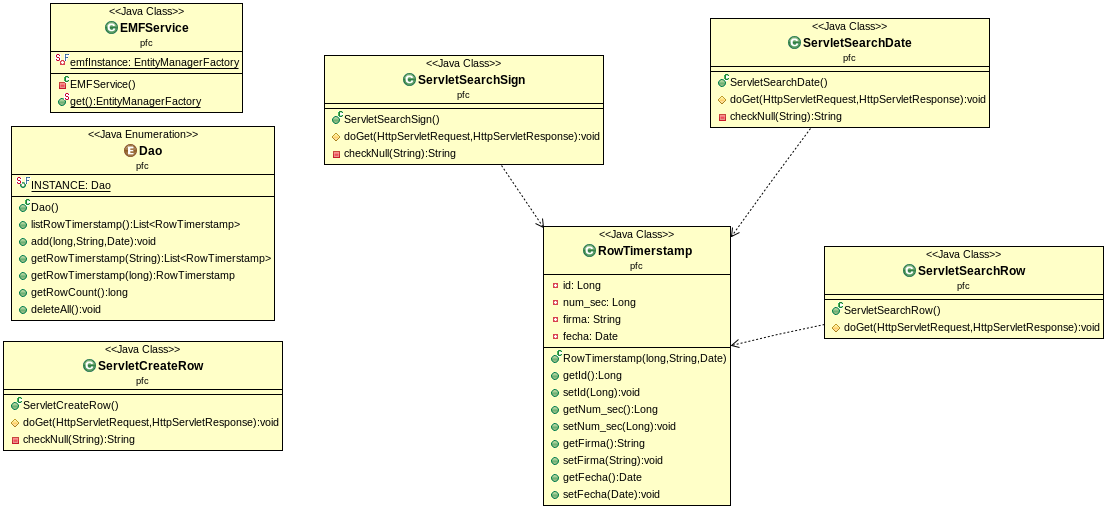
\includegraphics[scale=0.6]{./GoogleAppEngine/imagenes/UML_pfc.png}
  \caption{Detalles del paquete pfc}
  \label{fig:paquete_pfc}
\end{figure}

A continuación vamos a explicar una por una las clases desarrolladas para el funcionamiento del servidor de timestamp.

\begin{itemize}

\item \textbf{Dao.java:} esta clase es la encargada de todos los accesos a la base de datos, desde la inserción, el borrado y el listado de las filas, hasta consultas que se necesiten. Se puede ver que las sentencias que son listado de columnas se realizan con una sentencia SQL, se puede ver un ejemplo es el siguiente trozo de código:

\begin{lstlisting}[style=Java]
EntityManager em = EMFService.get().createEntityManager();
Query q = em.createQuery("select t from RowTimerstamp t where t.num_sec = :num_sec");
q.setParameter("num_sec", id);
RowTimerstamp RowTimerstamps = (RowTimerstamp)q.getSingleResult();
\end{lstlisting}

Pero las consultas que implican inclusión o borrado de filas no se realizan mediante sentencias SQL convencionales, se realizan con métodos que proporciona la API, un ejemplo es el siguiente trozo de código:

\begin{lstlisting}[style=Java]
EntityManager em = EMFService.get().createEntityManager();
RowTimerstamp RowTimerstamp = new RowTimerstamp(num_sec, firma, fecha);
em.persist(RowTimerstamp);
em.close();
\end{lstlisting}

\item \textbf{RowTimerstamp.java:} en esta clase se diseña el formato de las filas de la base de datos, que como se ha explicado anteriormente no se crea con sentencias SQL, se usa un modelo de programación llamado JPA. Para dicho modelo hay que crear una clase que contenga como variables de clase, las columnas que formarán la tabla en la base de datos. Como podemos ver, mediante un mecanismo llamado anotaciones Java, se le indica si el campo es la clave primaría, si es auto incrementado y otras opciones que habría que indicar en la creación de la tabla. A continuación podemos ver un trozo de código con las variables que posteriormente serán las filas de la tabla que queremos crear.  

\begin{lstlisting}[style=Java]
@Id
@GeneratedValue(strategy = GenerationType.SEQUENCE)
private Long id;
private Long num_sec;
private String firma;
private Date fecha;
\end{lstlisting}

Se puede ver que el campo \lstinline{id} será la clave primaría, que se indica mediante la anotación \lstinline{@Id} y que será auto incremental, a su vez también podemos ver el resto de datos que se van a almacenar, el campo \lstinline{num_sec} que es el número de secuencia, ya que el campo \lstinline{id} lo usa la base de datos para organizarse internamente, el campo \lstinline{firma} que es hash firmado por el usuario, el campo \lstinline{fecha} como su nombre indica es la fecha en la que se subió el hash firmado. El resto de métodos que tiene esta clase son un constructor, getter para consultar los campos y setter para insertar valores.

\item \textbf{ServletCreateRow.java:} esta clase es un servet que se encarga de recibir todos los parámetros necesarios y añadirlos a la base de datos. Al recibir los parámetros mediante \lstinline{GET} tiene que implementar el método \lstinline{doGet}, casi todos los servlets implementados en el proyecto mandan los parámetros mediante \lstinline{GET}. La forma de recibir parámetros es la siguiente:

\begin{lstlisting}[style=Java]
String firma = req.getParameter("firma");
\end{lstlisting}

El resto de parámetros que se necesitan se generan en el servidor para que no puedan ser falseados, como es el número de secuencia y la fecha. Si la inserción se produce correctamente se devuelve una cadena que tiene el siguiente formato: ``ok;;num\_sec;;fecha", que será interpretado en la aplicación móvil y parseará dicha cadena para conseguir los valores que necesitemos.

%Quitado porque se pueden borrar datos que queramos con el dashboard
%\item \textbf{ServletDeleteAll.java:} es un servlet ``secreto" que se usa para borrar todas las filas del servidor, cosa que no se debería poder para no poder falsear los datos introducidos en el servidor de timestamp. Hay que llamarlo con un parámetro que es \textbf{borrar} con valor \textbf{5}.

\item \textbf{ServletSearchDate.java:} es un servlet que devuelve una cadena con la fecha de una fila que tiene el número de secuencia que se le pasa en el parámetro \lstinline{token}.

\item \textbf{ServletSearchRow.java:} es un servlet que devuelve una página web donde se puede observar en una única fila con toda la información almacenada correspondiente al número de secuencia que se le pasa mediante el parámetro \lstinline{id}. A continuación se puede ver un trozo de código que lo realiza:

\begin{lstlisting}[style=Java]
PrintWriter pw = resp.getWriter();
pw.print("<!DOCTYPE html>");
pw.print("<html><head><title>Lista Time Stamp</title><link rel=\"stylesheet\" type=\"text/css\" " + "href=\"css/main.css\"/> <meta charset=\"utf-8\"> </head>");
pw.print("<body><table><tr><th>ID</th><th>Num sec</th><th>Firma</th><th>Date</th></tr><tr> " + "<td>"+ row.getId() +"</td><td>"+ row.getNum_sec() +"</td><td>"+ row.getFirma() +"</td><td>" +	row.getFecha() + "</td></tr> </table></body>");
pw.flush();
\end{lstlisting}

Como se puede ver se crea una tabla en una web, con la etiqueta \lstinline{<TABLE>} y su fila se rellena dinámicamente dependiendo del número de secuencia que se le pase como parámetro.

\item \textbf{ServletSearchSign.java:} Es un servlet que devuelve una cadena con la firma que corresponde al número de secuencia que se pasa por el parámetro \lstinline{token}.

\end{itemize}

La mayoría de estos servlets son usados por la otra aplicación web o por la aplicación móvil para realizar comprobaciones o mostrar información.

%TODO: falta los jsp

\subsection{Servidor de registro de firmas.}

El servidor de registro de firmas que hemos desarrollado es una aplicación web en la que los usuarios pueden consultar las firmas realizadas, las firmas de las que es destino, gestionar sus certificados de clave pública, verificar una firma realizada por otro usuario, exportar una cadena con la que cualquier usuario pueda consultar si la firma que has realizado es válida, que se usará en comprobaciones en caso de que ocurra algún problema y generar códigos QR para que que otros usuarios puedan firmarlo.

El sistema de gestión de usuarios lo proporciona Google y para entrar en la aplicación web hay que poseer una cuenta de Google Account, si no se está autentificado se produce una redirección a la página de autentificación, que la podemos ver en la figura~\ref{fig:logueoRepoGeneral}. La parte de la seguridad de los usuarios, autenticación y mantenimiento de las base de datos lo realiza Google.

\begin{figure}[h]
  \centering
    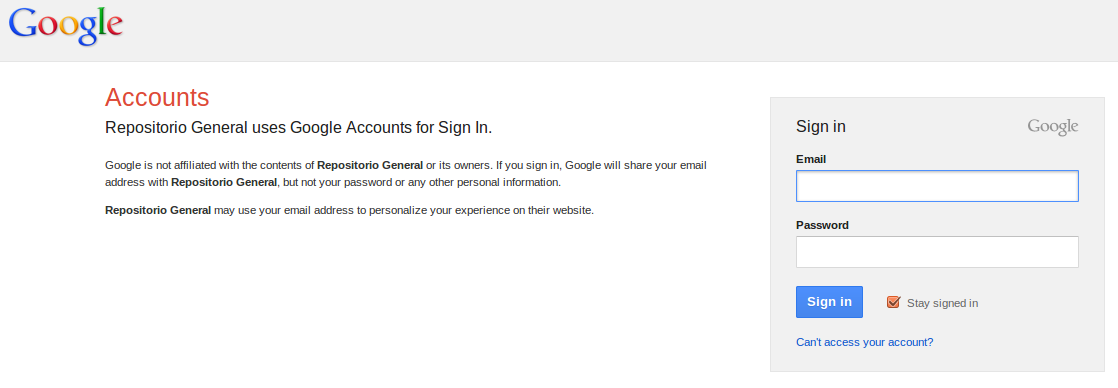
\includegraphics[scale=0.5]{./GoogleAppEngine/imagenes/login_repositorio_general.png}
  \caption{Login en Repositorio General}
  \label{fig:logueoRepoGeneral}
\end{figure}

La aplicación web se puede ver en la figura~\ref{fig:repositorio_general}, podemos ver que tiene varias pestañas, que se explicarán posteriormente, pero principalmente cada una de ellas se encarga de realizar una de las funciones que hemos comentado antes.

\begin{figure}[h]
  \centering
    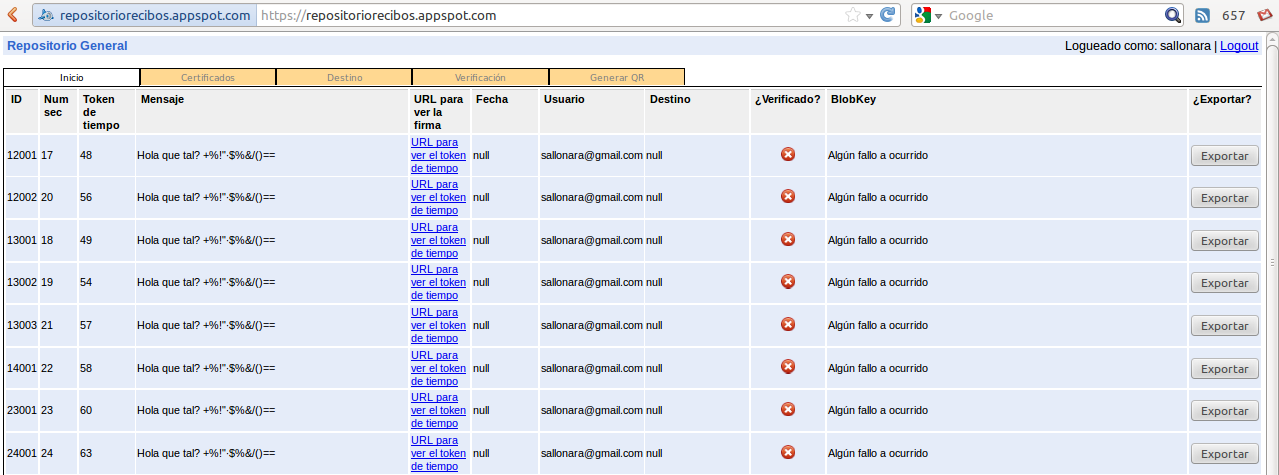
\includegraphics[scale=0.4]{./GoogleAppEngine/imagenes/repositorio_general.png}
  \caption{Repositorio General}
  \label{fig:repositorio_general}
\end{figure}

\subsubsection{Explicación de la aplicación web.}

%TODO: falta explicar como funciona la BD...
En la figura~\ref{fig:clasesReposotorioGeneral} se puede ver las clases que forman el paquete \textit{pfc} de la aplicación web repositorio general. A continuación vamos a explicar una por una las clases desarrolladas.

\begin{figure}[h]
  \centering
    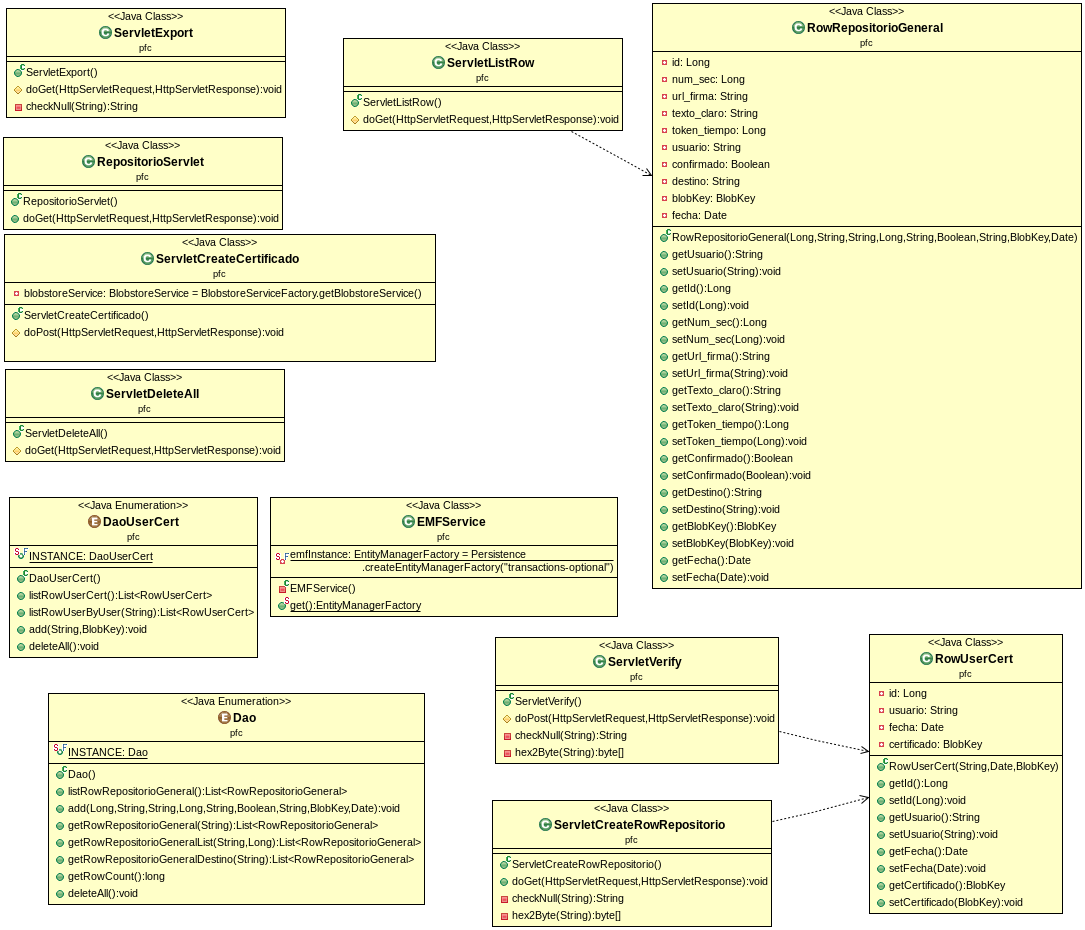
\includegraphics[scale=0.4]{./GoogleAppEngine/imagenes/UML_repositorio.png}
  \caption{Detalles de las clases Repositorio General.}
  \label{fig:clasesReposotorioGeneral}
\end{figure}

\begin{itemize}

\item \textbf{Dao.java:} al igual que en el servidor de timestamp, esta clase es la encargada de hacer todas las operaciones relacionadas con la base de datos.

\item \textbf{DaoUserCert.java:} como hemos implementado dos bases de datos, una para guardar las firmas y otra para guardar los certificados de clave pública que se necesitan, esta clase es la encargada de realizar todas las operaciones en la base de datos donde se guardan los certificados. 

\item \textbf{RowRepositorioGeneral.java:} esta es la clase con la que se crea la tabla en la que se almacenan las firmas de los usuario, tiene los siguientes campos:  

\begin{lstlisting}[style=Java]
@Id
@GeneratedValue(strategy = GenerationType.SEQUENCE) //	 GenerationType.IDENTITY
private Long id;
private Long num_sec;
private String url_firma;
private String texto_claro;
private Long token_tiempo;
private String usuario;
private Boolean confirmado;
private String destino;
private BlobKey blobKey;
private Date fecha;
\end{lstlisting}

Tiene una clave primaría \lstinline{id} que es usada por la base de datos internamente para el almacenado de la información, \lstinline{num_sec} es el número de secuencia dentro la tabla, que va incrementándose automáticamente, \lstinline{url_firma} es la dirección en la que se puede consultar la firma del texto en claro que está en el campo \lstinline{texto_claro}, se guarda el \lstinline{token_tiempo} que es el \lstinline{num_sec} de en la aplicación web servidor de timestamp. La columna \lstinline{usuario} almacena el usuario que ha realizado la firma, y en la columna \lstinline{destino} se guarda a quien va dirigida la firma. En la columna \lstinline{blobkey} se guarda la referencia al certificado de clave pública que estaba en activo cuando se subió la firma a la aplicación web, la columna \lstinline{confirmado} puede valer \lstinline{true} or \lstinline{false} e indica si al subir la firma se pudo verificar, en \lstinline{fecha} está la fecha en la que se almacenó.

\item \textbf{RowUserCert.java:} Esta clase es la encargada de crear la tabla que usamos para guardar los archivos con la clave pública. Los campos que usaremos para almacenarlos serán los que se pueden ver en el siguiente trozo de código.

\begin{lstlisting}[style=Java]
@Id
@GeneratedValue(strategy = GenerationType.SEQUENCE)
private Long id;
private String usuario;
private Date fecha;
private BlobKey certificado;
\end{lstlisting}

Como podemos ver el campo \lstinline{id} será la clave primaria y como hemos explicado será usado por la base de datos internamente para autogestión de las filas, el campo \lstinline{usuario} guardará una cadena con el email de la persona que ha subido ese archivo, el campo \lstinline{fecha} es la fecha en la que se subió el archivo, \lstinline{certificado} es un campo del tipo \lstinline{BlobKey} que es como la ruta al archivo de certificado.

\end{itemize}

Acto seguido vamos a explicar los diferentes servlets que hemos desarrollado para la aplicación web.

\begin{itemize}

\item \textbf{ServletCreateCertificate.java:} Este servlet es el encargado de añadir a la base de datos el certificado de clave pública. Es usado en la pestaña de certificados de la aplicación web y es llamado cuando se pulsa el botón subir certificado. Se puede observar dicho botón en la figura~\ref{fig:pestanhaCertificados}.

\end{itemize}

\begin{figure}[h]
  \centering
    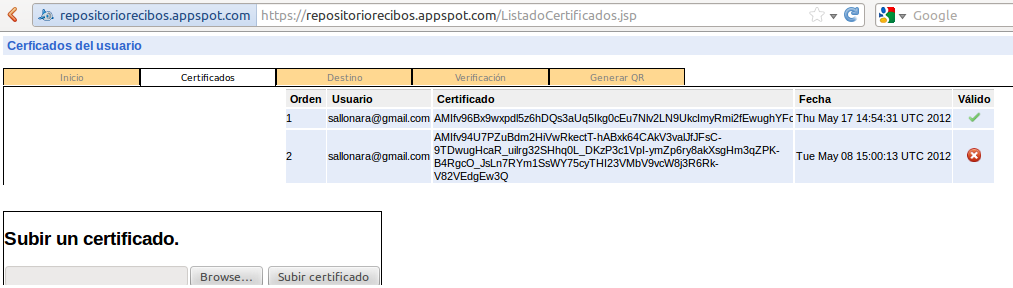
\includegraphics[scale=0.5]{./GoogleAppEngine/imagenes/certificadosRepositorioGeneral.png}
  \caption{Pantallazo de la pestaña certificados.}
  \label{fig:pestanhaCertificados}
\end{figure}

\begin{itemize}

\item \textbf{ServletCreateRowRepositorio.java:} Este servlet está mapeado en la dirección: \url{https://repositoriorecibos.appspot.com/add} y recibe los siguientes parámetros: \url{texto}, \url{url\_firma}, \url{token}, \url{destino} y \url{fecha}. Es el encargado de añadir una fila a la base de datos por cada llamada a dicha dirección, a esta dirección no hay forma de acceder desde la aplicación web. A su vez antes de introducir la fila comprueba que la firma se puede validar y se marca como \lstinline{true} o \lstinline{false} la columna verificado que posteriormente en el archivo \textit{RepositorioGeneralApplication.jsp} se cambiará por una imagen para hacer la verificación más visual. Si hemos podido insertar la fila, el servlet devuelve la cadena ``OK", si no se devuelven varias cadenas con los fallos que han ocurrido.

%\item \textbf{ServletDeleteAll.java:} Servlet ``secreto" que borra todas las filas de firmas almacenadas, hay que llamarlo con un parámetro que es \textit{borrar} con valor \textit{7}

\item \textbf{ServletExport.java:} Este servlet es el encargado de exportar una de las filas para que otra persona pueda comprobar si la firma es válida. Este servlet es llamado cuando se pulsa el botón exportar de la pestaña principal de la aplicación web. Se puede observar en la figura~\ref{fig:botonExportar}

\end{itemize}

\begin{figure}[h]
  \centering
    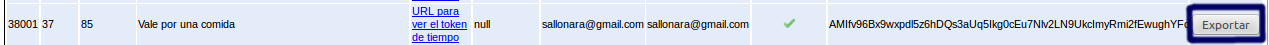
\includegraphics[scale=0.4]{./GoogleAppEngine/imagenes/botonExportar.png}
  \caption{Detalle del botón exportar.}
  \label{fig:botonExportar}
\end{figure}

\begin{itemize}

El servlet recibe los siguiente parámetros:

\begin{lstlisting}[style=Java]
String mensaje = checkNull(req.getParameter("mensaje"));
String url_firma = checkNull(req.getParameter("token"));
String id_blob = checkNull(req.getParameter("id_blob"));
String user = checkNull(req.getParameter("usuario"));
\end{lstlisting}

Una vez se tienen esos parámetros creamos una cadena de texto en la que unimos los siguiente campos y cada parámetro va separado por el separador: ``;/:".

\begin{lstlisting}[style=Java]
String cadACodificar = mensaje + ";/:" + url_firma + ";/:" + id_blob + ";/:" + user;
\end{lstlisting}

Acto seguido codificamos la cadena con \lstinline{Base64}\footnote{Para más información puede consultar: \url{http://en.wikipedia.org/wiki/Base64}}, que es una forma simple de codificar los caracteres para que no viajen en texto claro.

\begin{lstlisting}[style=Java]
String cadCodificada = Base64.encode(cadACodificar.getBytes("UTF-8"));
\end{lstlisting}

También añadimos unos limitadores para que cuando tengamos que decodificar ese mensaje podamos saber donde empiezan y donde termina la exportación.
\begin{lstlisting}[style=Java]
pw.println("BEGIN EXPORT");
pw.println("--------------------------");
pw.println(cadCodificada);
pw.println("--------------------------");
pw.println("END EXPORT");
\end{lstlisting}

\item \textbf{ServletListRow.java:} Este servlet es el encargado en devolver todas las filas de la tabla que pertenecen a un usuario. La forma de hacerlo es la siguiente, primero se identifica el usuario con el que se ha autentificado de esta forma:

\begin{lstlisting}[style=Java]
UserService userService = UserServiceFactory.getUserService();
User user = userService.getCurrentUser();
\end{lstlisting}

Una vez se consigue el usuario se llama a la función \lstinline{public List<RowRepositorioGeneral> getRowRepositorioGeneralList(String userId, Long num_sec)} de la clase \lstinline{Dao.java}, esta última función nos devuelve una lista con todas las filas. Al llamar al servlet le pasaremos el último número de secuencia que tenemos guardado en el teléfono móvil, para así agilizar las transferencias de datos, de esta forma solo nos devolverá las filas nuevas. La forma de devolvernos las filas será mediante una estructura llamada \lstinline{JSONArray}, que es un objeto que dentro contiene varios objetos \lstinline{JSON}\footnote{Para saber que es un objeto \lstinline{JSON} pueden consultar los siguientes enlaces: \url{http://www.json.org/} o \url{http://en.wikipedia.org/wiki/JSON}}.

La creación de los objetos \lstinline{JSON} la realizamos de la siguiente forma:

\begin{lstlisting}[style=Java]
JSONObject jsonObject = new JSONObject();

jsonObject.put("num_sec", rowRepositorioGeneral.getNum_sec().toString());
jsonObject.put("texto", rowRepositorioGeneral.getTexto_claro());
jsonObject.put("url_firma", rowRepositorioGeneral.getUrl_firma());
jsonObject.put("token_tiempo", rowRepositorioGeneral.getToken_tiempo().toString());
jsonObject.put("usuario",rowRepositorioGeneral.getUsuario());
jsonObject.put("fecha", rowRepositorioGeneral.getFecha().toString());
jsonObject.put("verificado", rowRepositorioGeneral.getConfirmado().toString());
jsonObject.put("destino", rowRepositorioGeneral.getDestino());
\end{lstlisting}

Ese objeto \lstinline{JSON} se añade un objeto \lstinline{JSONArray}, que es el que devolveremos como respuesta final de la ejecución de nuestro servlet y que espera la aplicación Android.

\item \textbf{ServletVerify.java:} Este servlet es el utilizado en la pestaña verificar de nuestra aplicación web, como se puede observar en la figura~\ref{fig:pestanhaVerificar}

\end{itemize}

\begin{figure}[h]
  \centering
    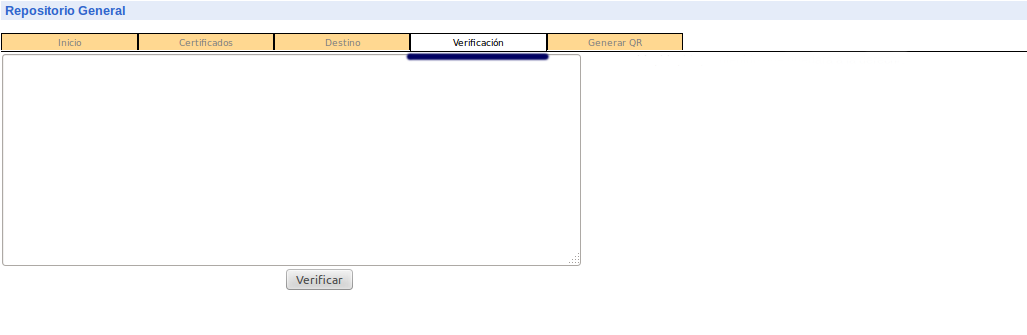
\includegraphics[scale=0.5]{./GoogleAppEngine/imagenes/pestanhaVerificar.png}
  \caption{Detalle de la pestaña verificación.}
  \label{fig:pestanhaVerificar}
\end{figure}

\begin{itemize}

\item Podemos observar que hay un cuadro de texto para introducir la cadena que devuelve el botón exportar. Cualquier usuario puede verificar si una firma es correcta o no. En este servlet se hace el proceso contrario que hicimos en exportar, quitamos los indicadores de inicio y final de exportación, desencriptamos la cadena en \lstinline{Base64} y hacemos varias comprobaciones. Comprobamos que en la fecha en la que se firmó el certificado era válido y que no habíamos revocado dicho certificado, también se comprueba que no fuera reemplazado por otro certificado antes de su expiración, ya que entonces la firma no sería válida. También comprobamos la integridad del mensaje, que la cadena no esté mal formada y que siga el formato que hemos obligado anteriormente.

\end{itemize}

Los archivos JSP que hemos creado en su mayoría solo rellenan tablas dinámicamente haciendo llamadas a funciones de la clase \lstinline{Dao.java}. Solo hay uno que no realiza esas funciones que es el siguiente:

\begin{itemize}

\item \textbf{GenerarQR.jsp:} Este archivo JSP es el que se muestra en la pestaña \textit{Generar QR}, se puede ver en la figura~\ref{fig:pestanhaQR}. Su función es generar un código QR para que pueda ser leído por la aplicación del móvil. Hay que rellenar los campos de destino y el texto que queremos que firme dicha persona. Al darle a \textit{Generar código QR} se hace una llamada a la API Google Chart y se genera un código QR que contiene dichas cadenas y se muestra en la parte de la derecha, como se puede ver en la figura~\ref{fig:codigoQR}.

\end{itemize}

\begin{figure}[h]
  \centering
    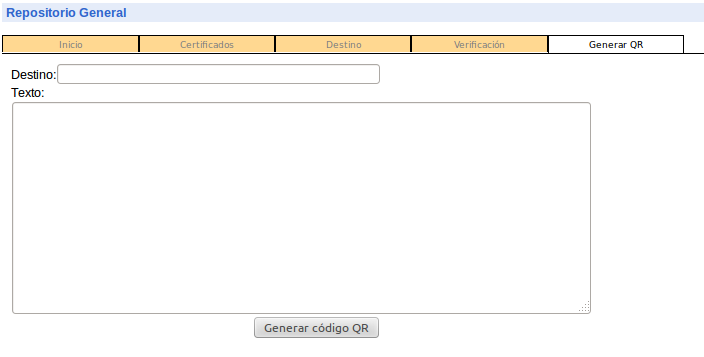
\includegraphics[scale=0.5]{./GoogleAppEngine/imagenes/pestanhaQR.png}
  \caption{Pestaña para generar el código QR.}
  \label{fig:pestanhaQR}
\end{figure}

\begin{figure}[h]
  \centering
    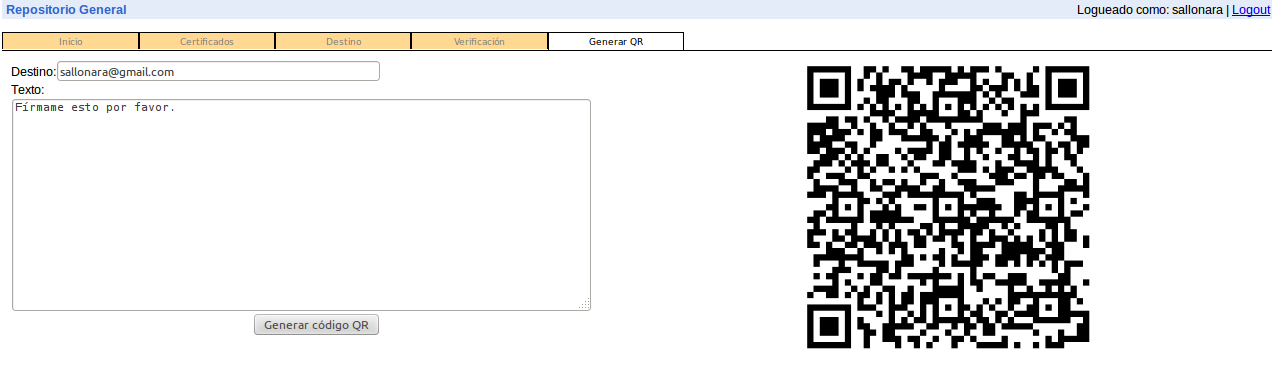
\includegraphics[scale=0.4]{./GoogleAppEngine/imagenes/codigoQR.png}
  \caption{Pestaña con el código QR generado.}
  \label{fig:codigoQR}
\end{figure}

